\documentclass[a4paper]{article}
\usepackage[left=2cm, right=2cm, bottom=2.5cm, top=2.5cm]{geometry}
\usepackage[utf8]{inputenc}
\usepackage{amsmath}
\usepackage{amsfonts}
\usepackage{amssymb}
\usepackage{commath}
\usepackage{lipsum}
\usepackage{adjustbox}
\usepackage{float}
\usepackage{hyperref}
\usepackage{graphicx}
\usepackage{gensymb}
\usepackage[spanish]{babel}

\usepackage{booktabs}

\title{\Huge{\vspace{-1em}Resumen FVV2}}
\author{\Large{\vspace{-1em}Alex Mart\'inez Ascensi\'on}}
\makeatletter
\let\newtitle\@title
\let\newauthor\@author
\makeatother

\usepackage{xcolor}

\usepackage{wrapfig}

\usepackage{fancyhdr}
\pagestyle{fancy}
\lhead{Alex Martínez Ascensión}
\chead{}
\rhead{\today}


\usepackage[T1]{fontenc}
\usepackage[default]{gillius}

\setlength{\parskip}{1em}
\setlength{\parindent}{0em}

\newcommand{\dd}{\ensuremath{\operatorname{d}}}
\renewcommand{\d}[1]{\ensuremath{\operatorname{d}\!{#1}}}

\begin{document}
	\maketitle




\section{Derivadas de orden superior; Máximos y mínimos}
\subsection{Teorema de Taylor}
Si recordamos el teorema para una variable, dada una función $f$ derivable $k$ veces en un punto $a$, entonces podemos escribir una aproximación de $f$ como:
\[ f(x) = f(a) + f'(a) (x-a) + \frac{f''(a)}{2!} (x-a)^2 + \cdots + \frac{f^{(k)}}{k!}(x-a)^k + R_k(x,a)\]
con $R_k$:
\[ R_k(x,a) = \int_a^x{\frac{(x-t)^k}{k!}f^{(k+1)}(t) \d t} \]

Así, conforme mayor es $k$, menor es $R_k$, y obtenemos una mejor aproximación de $f$.

Si desarrollamos el teorema para varias variables con derivadas hasta de tercer orden tenemos la expresión:
\[ f(\textbf{x}_0+\textbf{h}) = f(\textbf{x}_0) + \sum^n_i{h_i\frac{\partial f}{\partial x_i}(\textbf{x}_0)} + \frac{1}{2!} \sum^n_{i,j}{h_ih_j\frac{\partial f}{\partial x_i \partial x_j}(\textbf{x}_0)} + R_2(\textbf{h}, \textbf{x}_0) \]

Aquí cambiamos un poco la notación por conveniencia. Si definimos $\textbf{x} = \textbf{x}_0 + \textbf{h}$, entonces  $f(\textbf{x}_0+\textbf{h})$, donde $\textbf{x}_0$ sería el equivalente multidimensional de $a$, entonces $\textbf{h} = \textbf{x} - \textbf{x}_0$, que sería el equivalente multidimensional de $(x-a)$. Por tanto, la expresión final nos va a quedar en función de $\textbf{h}$.

La expresión anterior se puede expandir hasta el orden que deseemos, k:
\[ f(\textbf{x}_0+\textbf{h}) = f(\textbf{x}_0) + \sum^n_{m_1}{h_{m_1}\frac{\partial f}{\partial x_{m_1}}(\textbf{x}_0)} + \frac{1}{2!} \sum^n_{{m_1},{m_2}}{h_{m_1}h_{m_2}\frac{\partial^2 f}{\partial x_{m_1} \partial x_{m_2}}(\textbf{x}_0)} + \cdots \]\[+
\frac{1}{k!} \sum^n_{{m_1},{m_2},\cdots,{m_k}}{h_{m_1}h_{m_2}\cdots h_{m_k}\frac{\partial^k f}{\partial x_{m_1} \partial x_{m_2} \cdots\partial x_{m_k}}(\textbf{x}_0)}
+ R_k(\textbf{h}, \textbf{x}_0) \]

\subsection{Extremos de funciones con valores reales}
Si $U \subset \mathbb{R}^n$ es abierto, $f: U \subset \mathbb{R}^n \rightarrow \mathbb{R}$ es diferenciable y $\textbf{x}_\textbf{0} \in U$, y se cumple que  $\textbf{D}f(\textbf{x}_\textbf{0}) = 0$, entonces $\textbf{x}_\textbf{0}$ es un punto crítico de $f$. Por tanto, para hallar extremos críticos, realizamos la derivada de $f$ e igualamos a cero su matriz derivada. La condición que haga que todos los elementos de la matriz derivada sean 0 es un punto crítico.

Si suponemos que $f$ tiene derivadas de segundo orden, entonces el hessiano de $f$ en $\textbf{x}_0$ es:
\[ Hf(\textbf{x}_0)(\textbf{h}) = \frac{1}{2} \sum^n_{i,j}{h_ih_j\frac{\partial^2 f}{\partial x_i \partial x_j}(\textbf{x}_0)}\]

Esta expresión puede reescribirse en forma matricial como:
\[ H(\textbf{h}) = \frac{1}{2} \left[\begin{matrix}
h_1&h_2&\cdots &h_n
\end{matrix}\right] 
B
\left[\begin{matrix}
h_1\\h_2\\\cdots\\ h_n
\end{matrix}\right] \qquad \textbf{H} = B = \left[\begin{matrix}
\frac{\partial^2 f}{\partial x_1^2} & \frac{\partial^2 f}{\partial x_1 \partial x_2} &\cdots& \frac{\partial^2 f}{\partial x_1 \partial x_n} \\
\frac{\partial^2 f}{\partial x_2\partial x_1} & \frac{\partial^2 f}{ \partial x_2^2} &\cdots& \frac{\partial^2 f}{\partial x_2 \partial x_n} \\
\vdots & \vdots &\ddots& \vdots \\
\frac{\partial^2 f}{\partial x_n \partial x_1} & \frac{\partial^2 f}{\partial x_n \partial x_2} &\cdots& \frac{\partial^2 f}{ \partial x_n^2} \\
\end{matrix}\right] \]

Para saber si un punto crítico es un máximo, mínimo o punto silla, nos fijaremos en la matriz hessiana, \textbf{H}. El punto crítico será máximo cuando $\textbf{H}$ sea definida negativa, y mínimo cuando sea definida positiva. Si recordamos de álgebra, una matriz en base $\mathcal{B}$ puede transformarse a una base $\mathcal{B}^*$ aplicando transformaciones en filas y columnas, de modo que la matriz resultante es una diagonal. Así, si la matriz es definida positiva, será de la forma de la izquierda, y si es definida negativa es de la forma de la derecha.
\[\left[\begin{matrix}
+ & 0 & 0 & \cdots & 0\\
0 & + & 0 & \cdots & 0\\
0 & 0 & + & \cdots & 0\\
\vdots & \vdots & \vdots & \ddots & \vdots\\
0 & 0 & 0 & \cdots & +\\

\end{matrix}\right] \qquad\qquad
\left[\begin{matrix}
- & 0 & 0 & \cdots & 0\\
0 & - & 0 & \cdots & 0\\
0 & 0 & - & \cdots & 0\\
\vdots & \vdots & \vdots & \ddots & \vdots\\
0 & 0 & 0 & \cdots & -\\
\end{matrix}\right]
\]

Visto esto, el criterio de clasificación es el siguiente:
\begin{itemize}
	\item Si el punto crítico es un mínimo, entonces $\frac{\partial^2 f}{\partial x_1^2} > 0$ y el determinante de todas las submatrices es positivo.
	\item Si el punto crítico es máximo, entonces $\frac{\partial^2 f}{\partial x_1^2} < 0$ y el determinante de las submatrices alterna el signo ($D_1 <0, D_2>0, D_3<0, \cdots$).
	\item Si los determinantes no siguen que todos son positivos o alternantes, pero son mayores que cero, entonces tenemos un punto silla (la matriz no es ni definida positiva ni negativa).
	\item Si el determinante es cero, entonces no podemos aplicar el criterio y tenemos que analizar la función por otros métodos.
\end{itemize}


En algunas situaciones nos piden analizar los máximos y mínimos de una función $f$ restringida a un conjunto $U$. Entonces los pasos a seguir son:
\begin{enumerate}
	\item Localizar los puntos críticos en $U$. No hace falta saber si son máximos o mínimos.
	\item Localizar los puntos críticos en la región frontera de $U$.
	\item Calcular el valor de todos los puntos críticos, y seleccionar el mayor y el menor.
\end{enumerate}


\section{Extremos restringidos y multiplicadores de Lagrange}
En muchas ocasiones queremos maximizar/minimizar una función sujeta a ciertas condiciones. Si $f$ es la función que queremos optimizar, y $g$ es una función de restricción, definida en un conjunto de nivel $c$: $g(\textbf{x})  = c$, entonces si $f$ restringida en $g$ tiene un máximo/mínimo en $\textbf{x}_0$, entonces existe un número real $\lambda$ tal que $\boldsymbol{\nabla}f(\textbf{x}_0) = \lambda\boldsymbol{\nabla}g(\textbf{x}_0)$.

Si consideramos la función $h(\textbf{x},\lambda) = f(\textbf{x})- \lambda[g(\textbf{x})-c]$, entonces para hallar los puntos críticos tenemos que resolver el siguiente sistema de ecuaciones:
\[\begin{cases} 
\frac{\partial h}{\partial x_1} = 0 \iff \frac{\partial f}{\partial x_1} = \lambda \frac{\partial g}{\partial x_1}  \\ 
\frac{\partial h}{\partial x_2} = 0 \iff \frac{\partial f}{\partial x_2} = \lambda \frac{\partial g}{\partial x_2}  \\ 
\cdots\\
\frac{\partial h}{\partial x_n} = 0 \iff \frac{\partial f}{\partial x_n} = \lambda \frac{\partial g}{\partial x_n}  \\ 
\frac{\partial h}{\partial \lambda} = 0 \iff g(\textbf{x}) = c  \\ 
\end{cases}\]

Como tenemos $n+1$ incógnitas (las $n$ componentes de \textbf{x} y $\lambda$), entonces tenemos $n+1$ ecuaciones, siendo la última la propia restricción del enunciado.

En muchas ocasiones tenemos más de una restricción. En este caso podemos generalizar el problema a $k$ restricciones añadiendo las diferentes restricciones al sistema. La ecuación a igualar sería en este caso:
$$\boldsymbol{\nabla}f(\textbf{x}_0) = \lambda_1\boldsymbol{\nabla}g_1(\textbf{x}_0)+\lambda_2\boldsymbol{\nabla}g_2(\textbf{x}_0)+\cdots+\lambda_k\boldsymbol{\nabla}g_k(\textbf{x}_0)$$

El sistema de ecuaciones a resolver es, por tanto:
\[\begin{cases} 
\frac{\partial h}{\partial x_1} = 0 \iff \frac{\partial f}{\partial x_1} = \lambda \frac{\partial g}{\partial x_1}  \\ 
\frac{\partial h}{\partial x_2} = 0 \iff \frac{\partial f}{\partial x_2} = \lambda \frac{\partial g}{\partial x_2}  \\ 
\cdots\\
\frac{\partial h}{\partial x_n} = 0 \iff \frac{\partial f}{\partial x_n} = \lambda \frac{\partial g}{\partial x_n}  \\ 
\frac{\partial h}{\partial \lambda_1} = 0 \iff g_1(\textbf{x}) = c_1  \\ 
\frac{\partial h}{\partial \lambda_2} = 0 \iff g_k(\textbf{x}) = c_2  \\ 
\cdots\\
\frac{\partial h}{\partial \lambda_k} = 0 \iff g_k(\textbf{x}) = c_k \\ 
\end{cases}\]

Que en este caso es un sistema de $n+k$ ecuaciones con $n+k$ incógnitas.

Una vez obtengamos los puntos críticos del problema de optimización, tenemos que saber si son máximos o mínimos. Para ello empleamos el criterio del hessiano limitado. Tomando el determinante:
\[
|\overline{H}| = \left|\begin{matrix}
0 & -\frac{\partial g}{\partial x_1} & -\frac{\partial g}{\partial x_2} & \cdots & -\frac{\partial g}{\partial x_n} \\
-\frac{\partial g}{\partial x_1} & \frac{\partial^2 h}{\partial x_1^2} & \frac{\partial^2 h}{\partial x_1\partial x_2} & \cdots & \frac{\partial^2 h}{\partial x_1 \partial x_n}\\
-\frac{\partial g}{\partial x_2} & \frac{\partial^2 h}{\partial x_2\partial x_1} & \frac{\partial^2 h}{\partial x_2^2}  & \cdots & \frac{\partial^2 h}{\partial x_2 \partial x_n}\\
\vdots & \vdots & \vdots & \ddots & \vdots\\
-\frac{\partial g}{\partial x_n} & \frac{\partial^2 h}{\partial x_n\partial x_1} & \frac{\partial^2 h}{\partial x_n \partial x_n}  & \cdots & \frac{\partial^2 h}{\partial x_n^2}\\
\end{matrix} \right|
\]
Realizamos los subdeterminantes $k\times k$ para $k \ge 3 $ y aplicamos el criterio del hessiano al revés: si todos los subdeterminantes son negativos, entonces el punto crítico es un mínimo local, mientras que si los signos de los subdeterminantes se alternan, el punto crítico es un máximo local. Si $|\overline{H}| = 0$ entonces el criterio no es concluyente.

Para $k = 3 $ el criterio se simplifica a que si $|\overline{H}_2|  =
\left|\begin{matrix}
0 & -\frac{\partial g}{\partial x_1} & -\frac{\partial g}{\partial x_2}  \\
-\frac{\partial g}{\partial x_1} & \frac{\partial^2 h}{\partial x_1^2} & \frac{\partial^2 h}{\partial x_1\partial x_2} \\
-\frac{\partial g}{\partial x_2} & \frac{\partial^2 h}{\partial x_2\partial x_1} & \frac{\partial^2 h}{\partial x_2^2}\\
\end{matrix} \right|
> 0$ entonces es máximo local y si $|\overline{H}_2| < 0$ entonces es un mínimo local.

\section{Teorema de la función implícita e inversa}
El teorema particular de la función implícita dice que, si $F: \mathbb{R}^{n+1} \rightarrow \mathbb{R}$ tiene derivadas parciales continuas y se denotan los puntos de $F$ por $(\textbf{x}, z), \textbf{x} \in \mathbb{R}^n$, y en un punto $(\textbf{x}_\textbf{0}, z_0)$ se cumple que 

\[ \text{(1)} \quad F(\textbf{x}_\textbf{0}, z_0) = 0 \qquad\qquad \text{(2)} \quad \frac{\partial F}{\partial z} (\textbf{x}_\textbf{0}, z_0) \neq 0 \]

Entonces existe una bola $U$ que contiene a  $\textbf{x}_\textbf{0}$ en $\mathbb{R}^n$, y una vecindad $V$ de $z_0$ en $\mathbb{R}$ tal que existe una función $g$ que hace $z = g(\textbf{x})$, y que cumple que $F(\textbf{x}, g(\textbf{x})) = 0$ para todo $\textbf{x}$ en $U$. Si $F(\textbf{x}, z) = 0$ en todo $U$ y $V$, entonces $z = g(\textbf{x})$ y se cumple que
\[ D_\textbf{x}g(\textbf{x}) = - \frac{D_\textbf{x}F(\textbf{x}, z)}{\frac{\partial F}{\partial z} (\textbf{x}, z)} \qquad\qquad\qquad \frac{\partial g}{\partial x_i} = -\frac{\frac{\partial F}{\partial x_i} (\textbf{x}, z)}{\frac{\partial F}{\partial z} (\textbf{x}, z)} \quad i = 1, \cdots, n\]

El teorema particular de la función implícita puede extenderse al teorema general. En este caso pasamos de ``resolver'' $F(x_1, \cdots, x_n, z) = 0$ a resolver el sistema:

\[\begin{cases}
F_1(x_1, \cdots, x_n, z_1, \cdots, z_n) = 0\\
\cdots \\
F_m(x_1, \cdots, x_n, z_1, \cdots, z_n) = 0\\
\end{cases}  \]

El sistema es resoluble si se cumplen las condiciones siguientes:
\[ \text{(1)} \quad F_i(\textbf{x}_\textbf{0}, \textbf{z}_\textbf{0}) = 0 \quad \forall \;\; i = 1,\cdots, m\qquad\qquad \text{(2)} \quad \Delta =  \left|\begin{matrix}
\frac{\partial F_1}{\partial z_1} & \cdots & \frac{\partial F_1}{\partial z_m}\\
 \vdots & & \vdots \\
 \frac{\partial F_m}{\partial z_1} & \cdots & \frac{\partial F_m}{\partial z_m}\\
\end{matrix} \right|_{(\textbf{x}_\textbf{0}, \textbf{z}_\textbf{0})}  \neq 0 \]

Entonces, se verifica que existen las funciones $z_1(\textbf{x}), \cdots, z_m(\textbf{x})$
que verifican el sistema de ecuaciones anterior. Además, si se realiza la derivación de las funciones:
\[\begin{cases}
\frac{\partial}{\partial x_1}F_1(x_1, \cdots, x_n, z_1(x_1, \cdots, x_n), \cdots, z_n(x_1, \cdots, x_n)) = 0\\
\cdots \\
\frac{\partial}{\partial x_m}F_1(x_1, \cdots, x_n, z_1(x_1, \cdots, x_n), \cdots, z_n(x_1, \cdots, x_n)) = 0\\
\cdots \\
\frac{\partial}{\partial x_1}F_m(x_1, \cdots, x_n, z_1(x_1, \cdots, x_n), \cdots, z_n(x_1, \cdots, x_n)) = 0\\
\cdots \\
\frac{\partial}{\partial x_m}F_m(x_1, \cdots, x_n, z_1, \cdots, z_n) = 0\\
\end{cases} 
\]

Y se resuelve el sistema correspondiente, se obtienen los valores de las derivadas parciales en el punto \textbf{x}.
\subsection{Función inversa}
Un caso particular de la función implícita sucede cuando tenemos sólo $f$ en funciones del sistema:
\[\begin{cases}
f_1(z_1, \cdots, z_n) = y_1\\
\cdots \\
f_m(z_1, \cdots, z_n) = y_n\\
\end{cases}  \]

Es decir, tenemos $y_1(z_1, \cdots, z_n), \cdots y_n(z_1, \cdots, z_n)$ y nos gustaría expresar el sistema como 
$z_1(y_1, \cdots, y_n), \cdots, z_n(y_1, \cdots, y_n)$. En otras palabras, buscamos las funciones inversas de $y_1, \cdots, y_n$. Según el teorema de la función inversa, esta inversión sucede en un punto $\textbf{z}_\textbf{0}$ si
\[ \Delta = \left| \frac{\partial(y_1, \cdots, y_n)}{\partial(z_1,\cdots, z_n)} \right|_{\textbf{z}_\textbf{0}} =  
\left|\begin{matrix}
\frac{\partial y_1}{\partial z_1} & \cdots & \frac{\partial y_1}{\partial z_n}\\
\vdots & & \vdots \\
\frac{\partial y_n}{\partial z_1} & \cdots & \frac{\partial y_n}{\partial z_n}\\
\end{matrix} \right|_{\textbf{z}_\textbf{0}} = 
\left|\begin{matrix}
\frac{\partial f_1}{\partial z_1} & \cdots & \frac{\partial f_1}{\partial z_n}\\
\vdots & & \vdots \\
\frac{\partial f_n}{\partial z_1} & \cdots & \frac{\partial f_n}{\partial z_n}\\
\end{matrix} \right|_{\textbf{z}_\textbf{0}} \neq 0 \]

\section{Funciones con valores vectoriales}
\subsection{Trayectorias y velocidad}
Una trayectoria es una función $\boldsymbol{\sigma}:[a,b] \rightarrow \mathbb{R}^n$. Los puntos $\boldsymbol{\sigma}(a)$ y $\boldsymbol{\sigma}(b)$ son los extremos de la trayectoria. La imagen de la trayectoria en $\mathbb{R}^n$ se llama curva. 

Así, una trayectoria $\boldsymbol{\sigma}(t)$ puede definirse en $\mathbb{R}^3$ como una función $\boldsymbol{\sigma}(t) = (x(t), y(t), z(t))$. La derivada de la trayectoria viene definida como:
\[ \boldsymbol{\sigma}'(t) = \lim_{h \rightarrow 0}\frac{\boldsymbol{\sigma}(t_0+h)-\boldsymbol{\sigma}(t_0)}{h} = (x'(t), y'(t), z'(t)) \]

La recta tangente a una trayectoria es $\textbf{l}(\lambda) = \boldsymbol{\sigma}(t_0) + \lambda\boldsymbol{\sigma}'(t_0)$

A nivel físico, si tenemos una trayectoria $\textbf{r}(t)$, a velocidad es $\textbf{v}(t)=\textbf{r}'(t)$, la rapidez es $S(t) = \Vert\textbf{v}(t)\Vert$ y la aceleración es $\textbf{a}(t) = \textbf{r}''(t)$.

\subsection{Longitud de arco}
Si tenemos una trayectoria $\boldsymbol{\sigma}:[a,b] \rightarrow \mathbb{R}^n$, la longitud de arco entre $a$ y $b$ está definida como:
\[ l(\boldsymbol{\sigma}) = \int^a_b{\Vert\boldsymbol{\sigma}'(t)\Vert \d t} = \int^a_b{\sqrt{ [x_1'(t)]^2+[x_2'(t)]^2+\cdots+[x_n'(t)]^2 }} \d t \]

Por lo general no nos interesa obtener la longitud de arco entre dos puntos, sino dado un $a$ fijo, obtener una función de longitud de arco para un tiempo $t$:
\[  s(t) = \int_a^t{\Vert\boldsymbol{\sigma}'(\tau)\Vert \d \tau} \]

Así, por el Primer Teorema del Cálculo, tenemos que $s'(t) = \Vert\boldsymbol{\sigma}'(t)\Vert$

\subsection{Campos vectoriales}
Un campo vectorial en $\mathbb{R}^n$ es una función $\textbf{F}: A  \subset \mathbb{R}^n \rightarrow \mathbb{R}^m$ que asigna a cada vector $\textbf{x}$ en $A$ su vector $\textbf{F}(\textbf{x})$ en $\mathbb{R}^m$. Así, por ejemplo, para una partícula posicionada en $\textbf{r}  =(x,y,z)$, su fuerza de atracción localizada en el origen es un campo vectorial $\textbf{F} = - \frac{mMG}{\Vert\textbf{r}\Vert^3}\textbf{r}$.

Una línea de flujo para $\textbf{F}$ es una trayectoria $\boldmath{\sigma}(t)$ tal que 
\[ \boldsymbol{\sigma}'(t) = \textbf{F}(\boldsymbol{\sigma}(t)) \]
Es decir, el argumento del campo vectorial es la propia trayectoria, y su imagen ha de ser igual a la derivada de la trayectoria. En condiciones iniciales, tomamos $\boldsymbol{\sigma}(0) = (x_0, y_0, z_0)$.

Para agilizar la notación, definimos $\phi(\textbf{x}, t)$ como la posición del punto en la línea de flujo tras haber transcurrido un tiempo $t$. Así, la ecuación anterior se reescribe como (además de una segunda condición inicial):
\[ \phi(\textbf{x}, 0) = \textbf{x} \qquad \frac{\partial}{\partial t} \phi(\textbf{x}, t)  \]

\subsection{Divergencia y rotacional de un campo vectorial}
Usualmente tomamos el gradiente como una función asociada a una función. Sin embargo, el gradiente como tal es un operador, es decir, un elemento matemático que combinado a una función modifica sus valores. Así, el gradiente como tal está definido como:
\[ \boldsymbol{\nabla}  = \textbf{i}\frac{\partial}{\partial x} + \textbf{j}\frac{\partial}{\partial y} + \textbf{k}\frac{\partial}{\partial z}\]

Y cuando hacemos $\nabla f$ en realidad hacemos el producto escalar entre $\boldsymbol{\nabla} $ y $f$.

La \textit{operación rotacional} asocia a cada campo vectorial $C^1$ $\textbf{F}$ el siguiente campo vectorial:
\[ \text{rot } \textbf{F} = {\boldsymbol{\nabla}} \times \textbf{F} = \left| \begin{matrix}
\textbf{i} & \textbf{j} & \textbf{k} \\
\frac{\partial}{\partial x} & \frac{\partial}{\partial y}  & \frac{\partial}{\partial z}  \\
F_1 & F_2 & F_3 \\
\end{matrix}\right| 
\]

Si ${\boldsymbol{\nabla}} \times \textbf{F}=0$, entonces decimos que $\textbf{F}$ es irrotacional.

Otra función es la \textit{divergencia} de un campo vectorial, definida como:
\[  \text{div } \textbf{F} = {\boldsymbol{\nabla}} \cdot \textbf{F} = \frac{\partial F_1}{\partial x} + \frac{\partial F_2}{\partial y} + \frac{\partial F_3}{\partial z} \]

En este campo, la divergencia es un campo escalar, a diferencia del rotacional, que es un campo vectorial.

Como ``curiosidad'', es importante recordar que la divergencia de un rotacional siempre es 0: 
\[ {\boldsymbol{\nabla}} \cdot ({\boldsymbol{\nabla}} \times \textbf{F}) = 0\] 

\rule{\linewidth}{1pt}

Además del operador gradiente existen otros muchos. Uno de los más importantes es el \textit{operador laplaciano}, definido como
\[ \Delta f = (\nabla\cdot\nabla)f = \nabla^2f = \sum^n_i\frac{\partial^2f}{\partial x_i^2} \]
Cuando una función cumple que su laplaciano es nulo, es decir, $\nabla^2f = 0$ decimos que es una \textit{función armónica}.

\section{Integrales dobles}
Dada una función $f: R \in \mathbb{R}^2 \rightarrow \mathbb{R}$, la integral doble de $f$ en $R$, denotada por 
\[\int_R f \qquad \int_R f(x,y) \d{A} \qquad \int_R f(x,y) \d{x}\d{y} \qquad \int\int_Rf(x,y) \d{x}\d{y} \]

Esta región denota el volumen entre el plano $z=0$ y la superficie generada por la función $f$ en $R$.

El principio de Cavalieri nos dice que si tenemos una figura, y sección transversal en $x$ es $A(x)$; si los extremos de la figura en $x$ son $a$ y $b$ ($a<x<b$)  entonces el volumen de la figura será:
\[ \int_a^b A(x) \d{x} \]

Así pues, si $A(x)$ está definida de manera integral entre $c$ y $d$, entonces
\[V = \int_a^b A(x) \d{x} = \int_a^b\left[\int_c^d f(x,y) \d{y}\right]\d{x} \]

Para regiones rectangulares, el teorema de Fubini nos permite cambiar el orden de integración sin alterar el valor de la integral, es decir:
\[V = \int_a^b\left[\int_c^d f(x,y) \d{y}\right]\d{x} =  \int_c^d\left[\int_a^b f(x,y) \d{x}\right]\d{y} \]

En muchas ocasiones las regiones son rectangulares, en cuyo caso $a$, $b$, $c$ y $d$ son escalares. Sin embargo, es posible que las regiones vengan dadas por una función. Si la región es de tipo I, entonces la región delimitada entre $a < x < b$ viene dada por dos funciones: $c = \phi_1(x) < y < d = \phi_2(x)$. Por otra parte, si la región es de tipo II, entonces para $c < y < d$ existen dos funciones tales que $a = \psi_1(y) < x < b=\psi_2(y)$. Las regiones de tipo III incluyen regiones de tipo I y II.

Así, la integral resultante puede representarse con las siguientes funciones tal que:
\[V = \int_{\phi_1(x)}^{\phi_2(x)}\int_{\psi_1(y)}^{\psi_2(y)} f(x,y) \d{y}\d{x}  \]

Para este tipo de integrales también se cumple un análogo del Teorema de Fubini, que es el cambio de orden de integración. Si hallamos sendas funciones tales que $\psi^*_1(x) = \psi_1^{-1}(y)$, $\psi^*_2(x) = \psi_2^{-1}(y)$, $\phi^*_1(y) = \phi_1^{-1}(x)$, $\phi^*_2(y) = \phi_2^{-1}(x)$ entonces:
\[V = \int_{\phi_1(x)}^{\phi_2(x)}\int_{\psi_1(y)}^{\psi_2(y)} f(x,y) \d{y}\d{x} =  \int_{\psi_1^*(x)}^{\psi_2^*(x)}\int_{\phi_1^*(x)}^{\phi_2^*(x)} f(x,y) \d{x}\d{y} \]

En otras palabras, si conseguimos hallar las funciones inversas que permitan invertir los ejes ($x, y$, en este caso) entonces el valor de la integral no cambia.

\subsection{Propiedades de la integral, y otros teoremas}
Similar al cálculo de una variable, para integrales múltiples se cumplen una serie de propiedades.
\begin{itemize}
	\item Linealidad 
	\[ \int_R[f(x,y)+g(x,y) ]\d{A} = \int_Rf(x,y)\d{A} + \int_R g(x,y) \d{A} \]
	\item Homogenei\d{A}d 
	\[ \int_R cf(x,y)\d{A} = c\int_Rf(x,y)\d{A} \]
	\item Monotonía: Si $f(x,y) \ge g(x,y) \ge 0$, entonces
	\[ \int_R f(x,y) \d{A} \ge \int_R g(x,y) \d{A} \]
	\item Aditivi\d{A}d: Si $R_1$, $R_2$, ..., $R_n$ son regiones disjuntas, es decir $R_i \cap R_j = \emptyset$ para todo $i \neq j$, entonces, si $Q = \bigcup_i R_i$:
	\[ \int_Q f(x,y) \d{A} = \sum_i \int_{R_i} f(x,y) \d{A} \]
	\item Valor absoluto
	\[ \left| \int_R f(x,y) \d{A} \right| \le \int_R \abs{f(x,y)} \d{A}  \]
\end{itemize}

El teorema del valor intermedio de una variable es extrapolable al de dos. Es decir, dada $f:D\rightarrow\mathbb{R}$, entonces en algún punto $(x_0, y_0)$ se cumple que 
\[ \int_D f(x,y) \d{A} = f(x_0, y_0) A(D) \]

\section{Integral triple, fórmula de cambio de variables y aplicaciones}
La notación de la integral triple es igual a la de la doble, sólo que con un integrando más. La integral puede realizarse sobre un volumen rectangular o, similar al caso de dos variables, con funciones $\phi$, $\psi$ y $\gamma$. Así, tenemos que un volumen está en una región de tipo I si $z = f(x,y)$, de tipo II si $x = f(y,z)$ y de tipo III si $y = f(x,z)$ (el resto de variables, para cada caso, estarían delimitadas por planos rectos). Finalmente, una región de tipo IV combina regiones de tipo I, II y III, de modo que se pueden generar figuras con múltiples ecuaciones, y poder hallar dicho volumen tal que:
\[ V = \int^{\gamma_2}_{\gamma_1}\int^{\phi_2}_{\phi_1}\int^{\psi_2}_{\psi_1} \d{v} \]

En este caso no indico cada función sobre qué variables está descrita porque eso dependerá del tipo de región que sea, que determina el orden de integración (es decir, $\d{x} \d{y} \d{z}$, $\d{z} \d{x} \d{y}$, etc.).

Por ejemplo, si la función fuera de tipo I, entonces el volumen sería
\[V = \int _ { a } ^ { b } \int _ { \phi _ { 1 } ( x ) } ^ { \phi _ { 2 } ( x ) } \int _ { \gamma _ { 1 } ( x , y ) } ^ { \gamma _ { 2 } ( x , y ) } \d{z}\d{y}\d{x}\]

Si a una integral triple le aplicamos una integración sobre una función $f(x,y,z)$, entonces estaríamos hallando la ``densidad'' del volumen en función de $f$. Si $f=1$ entonces la densidad es constante, y obtenemos el volumen a secas.

\subsection{Teorema del cambio de variable}
Sean $D$ y $D^*$ regiones elementales del plano, y sea $T:D^*\rightarrow D$ una función $C^1$ e inyectiva en $D$, de modo que $T(D^*) = D$. Entonces, para cualquier función $F:D\rightarrow \mathbb{R}$ se cumple que
\[ \int_Df(x,y) \d{x}\d{y} = \int_{D^*} f(x(u,v), y(u,v)) \left|\frac{\partial(x,y)}{\partial(u,v)}\right|\d{u}\d{v} \]

Donde $\left|\frac{\partial(x,y)}{\partial(u,v)}\right|$ es el jacobiano definido por 
\[ \left|\frac{\partial(x,y)}{\partial(u,v)}\right| = \left|
\begin{matrix}
\frac{\partial x}{\partial u} & \frac{\partial x}{\partial v} \\
\frac{\partial y}{\partial u} & \frac{\partial y}{\partial v} \\
\end{matrix}\right| \]

Este teorema de dos variables puede extenderse a $n$ dimensiones, tal que si tanto $D$ como $D^* \in \mathbb{R}^n$ entonces:
\[ \int_Df(\alpha, \beta, \cdots, \omega) \d{\alpha}\d{\beta}\cdots\d{\omega} = \int_{D^*} f(\alpha(A, B, \cdots, \Omega), \cdots, \omega(A, B, \cdots, \Omega))\left|\frac{\partial(A, B, \cdots, \Omega)}{\partial(\alpha, \beta, \cdots, \omega)}\right| \d{\alpha}\d{\beta}\cdots\d{\omega}  \]

La intuición detrás del uso del jacobiano es que éste indica cual es el volumen n-dimensional de los vectores $T_A$, $T_B$, $\cdots$, $T_\Omega$, que serían tangentes a un punto en la región $D^*$. Así pues, el jacobiano indica cual es el cambio de volumen entre $D^*$ y $D$, de modo que multiplicando por el jacobiano igualamos la escala de volumen entre ambas superficies.

\subsection{Aplicaciones de la integral}
A continuación resumimos en una tabla las principales aplicaciones para las integrales múltiples. Incluimos entre las aplicaciones el promedio, el centro de masa, y el momento de inercia. En los dos primeros casos añadimos el caso discreto y el continuo en una variable para mostrar el trasfondo del caso multivariable.

\begin{center}
\begin{tabular}{lccc} \midrule
	& Modelo discreto & Modelo continuo (1v) & Modelo continuo (>1v)\\ \midrule
	Promedio & $\overline{x} = \frac{\sum_i f(x_i)}{n}$ &
	$f_{prom} = \frac{\int_a^bf(x) \d{x}}{b-a}$ & 
	$f_{prom} = \frac{\iint_D f(x_1, \cdots, x_n) \d{A}}{\iint_D\d{A}}$ \\
	& & & \\
	\small{Centro de masa} & $\sum_i(x_i-\overline{x})m_i = 0 \;\;\; \overline{x} = \frac{\sum_ix_im_i}{\sum_im_i}$ & 
	$\overline{x} = \frac{\int x f(x) \d{x}}{\int f(x) \d{x}}$ &
	$x_i = \frac{\iint_D x_i f(x_1,\cdots,x_i,\cdots,x_n)\d{A}}{\iint_D f(x_1,\cdots,x_i,\cdots,x_n)\d{A}}$\\
	& & & \\
	\small{Momento de inercia} &
	$I_x = k \iiint_W y^2+z^2 \d{x}\d{y}\d{z}$ &  
	$I_y = k \iiint_W x^2+z^2 \d{x}\d{y}\d{z}$ & 
	$I_z = k \iiint_W y^2+x^2 \d{x}\d{y}\d{z}$ \\
	
	 \midrule
\end{tabular}
\end{center}

 \subsection{Integrales impropias}
Al igual que con las funciones de una variable, en funciones de varias variables podemos tener situaciones donde nos interese evaluar la integral en $\pm \infty$ o en un punto $a \in \mathbb{R}^n$ donde $f(a) = \infty$. 

Supongamos (en dos variables por hacerlo simple) que tenemos la siguiente integral:
\[ \int_D f \d{A} = \int_{\phi_{ 1 }(x)}^{\phi_{2}(x)}\int_{\psi_{ 1 }(y)}^{\psi_{2}(y)} f(x,y) \d{y}\d{x} \]

Y la integral es impropia. Pongamos que es una integral impropia del tipo $f(a) = \infty$. Entonces, para resolver la integral, podemos crear la siguiente integral:
\[ \int_{D_{\eta,\delta}} f \d{A} = \int_{\phi_{ 1 }(x)-\eta}^{\phi_{2}(x)+\eta}\int_{\psi_{ 1 }(y)-\delta}^{\psi_{2}(y)+\delta} f(x,y) \d{y}\d{x} \]

Y evaluamos el limite 
\[ \lim_{\eta,\delta} \int_{D_{\eta,\delta}} f \d{A} \]

Para saber si la integral converge o diverge. En los casos en los que la integral tiene uno de los límites en $\pm \infty$, por ejemplo:
\[\int_a^b\int_{\psi_{ 1 }(y)}^{+\infty} f(x,y) \d{y}\d{x} \]

Hacemos el límite
\[ \lim_{\delta \rightarrow +\infty} \int_a^b\int_{\psi_{ 1 }(y)}^{\delta} f(x,y) \d{y}\d{x}\]
Para evaluar la integral.

De igual modo que para una variable, para funciones de varias variables se cumplen ciertos teoremas sobre integrales impropias.

Sea $0 \le g(x,y) \le f(x,y)$. Si $\int_D f(x,y) \d{A}$ es finita, entonces $\int_D g(x,y) \d{A}$ también lo es. Por otra parte, si $\int_D g(x,y) \d{A}$ no existe (es infinito), entonces $\int_D f(x,y) \d{A}$ tampoco.



\section{Integrales de trayectoria y superficies}
\subsection{Integral de trayectoria y de línea}
Una trayectoria $\sigma$ queda definida como la función de clase $C^1$ $\sigma: I = [a,b] \in \mathbb{R} \rightarrow \mathbb{R}^3$ donde $\boldsymbol{\sigma}(t) = (x(t), y(t), z(t))$. Así, la integral de trayectoria sobre una función $f(x,y,z)$ viene definida por:
\[ \int_{\boldsymbol{\sigma}} f \d{s} = \int_a^b f(x(t), y(t), z(t)) \lVert\boldsymbol{\sigma}'(t)\rVert \d{t} \]

Si $f(x,y,z) = 1$, entonces estaríamos calculando la longitud de arco de la trayectoria. Así, la integral de trayectoria define, de manera informal, el área que genera $f$ sobre $\sigma$, como si de una pared se tratase.

Si nos fijamos, una integral de linea trabaja sólo con escalares: tanto $f(x,y,z)$ como $\Vert\boldsymbol{\sigma}'(t)\Vert$ son funciones en $\mathbb{R}$. Si queremos extender estas funciones en $\mathbb{R}^3$ (o $\mathbb{R}^n$), recurrimos al concepto de integral de línea. 

Si definimos $F$ como un campo vectorial en $\mathbb{R}^3$ continuo en $\sigma$, entonces la integral de línea de $F$ en $\sigma$ queda definida como:
\[ \int_\sigma F \d{s} = \int_a^b F(\sigma(t))\cdot \boldsymbol{\sigma}'(t) \d{t} \]

Otra forma de representar $\int_\sigma F \d{s}$ es basándonos en el vector unitario de $\sigma'(t)$:
\[ \int_\sigma F \d{s} = \int_a^b \left[F(\boldsymbol{\sigma}(t))\cdot\frac{\boldsymbol{\sigma}'(t)}{\Vert\boldsymbol{\sigma}'(t)\Vert} \right] \Vert\boldsymbol{\sigma}'(t)\Vert \d{t} = \int_a^b [F(\boldsymbol{\sigma}(t)·T(t)]\Vert\boldsymbol{\sigma}'(t)\Vert \d{t} \]

La integral de línea nos vendría a decir la cantidad de "fuerza" total ejercida por $F$ a lo largo de $\sigma$. Por ejemplo, si $\sigma$ es perpendicular a $F$ en todo momento, entonces $\boldsymbol{\sigma}'(t) \perp F(\boldsymbol{\sigma}(t))\iff\boldsymbol{\sigma}'(t) \cdot F(\boldsymbol{\sigma}(t)) = 0 \iff \int_\sigma F \d{s} = 0 \;\; (F, \boldsymbol{\sigma} \neq 0)$

Una de las propiedades de integrales de línea es que son independientes de reparametrizaciones. Una reparametrización es la composición de dos funciones: $\sigma$, la trayectoria original, y $h$ una función transformadora. Si $h: I \rightarrow J$ es de clase $C^1$ y $\sigma: J \rightarrow \mathbb{R}^3$, entonces $\rho : I \rightarrow \mathbb{R}^3$ es $\boldsymbol{\rho} = \boldsymbol{\sigma}(h) = \sigma \circ h$. Si tanto $h$ como $\sigma$ son inyectivas, entonces $\rho$ también es inyectiva, y podemos aplicar la integral de linea sobre $\rho$.

Si aplicamos el teorema de cambio de variable, teniendo en cuenta que $\boldsymbol{\rho}(t) = \boldsymbol{\sigma}(h(t)) \iff \boldsymbol{\rho}'(t) = \boldsymbol{\sigma}'(h(t))\cdot h'(t)$, entonces podemos hacer $s = h(t)$ y podemos demostrar que
\[ \int_{h(a)}^{h(b)}F(\boldsymbol{\sigma}(s))\cdot\boldsymbol{\sigma}'(s) \d{s} = \int_a^b F(\boldsymbol{\sigma}(h(t)))\cdot\boldsymbol{\sigma}'(h(t))\cdot h'(t) \d{t} = \int_a^b F(\boldsymbol{\rho}(t)) \cdot \boldsymbol{\rho}'(t) \d{t} \]

Si $\rho$ preserva la orientación, es decir si $I = [a,b]$ entonces $\rho : [\sigma(a), \sigma(b)] \rightarrow\mathbb{R}^3$, entonces $\int_\rho F \d{s} = \int_\sigma F \d{s}$, mientras que si $\rho$ invierte la orientación, es decir, $\rho : [\sigma(b), \sigma(a)]\rightarrow\mathbb{R}^3$, entonces $\int_ \rho F \d{s} = -\int_\sigma F \d{s}$. 

Esta reparametrización también se cumple para $f$ en integrales de trayectoria. Sin embargo, la integral no cambia de signo aunque se invierta la orientación.

Si $\rho$ (o $\sigma$) tienen puntos donde no son continuas, o no son diferenciables, entonces, pero la trayectoria puede dividirse en subtrayectorias diferenciables, entonces la integral de la trayectoria es igual a la suma de las integrales de las subtrayectorias:
\[ C = \bigcup_i C_i \iff \int_C \sigma \d{s} = \sum_i \int_{C_i} \sigma \d{s} \]

Por último, relacionamos el segundo teorema fundamental del cálculo con las integrales de trayectoria. Recordamos que el teorema dice que si $H' = h$ y $H(x) = \int_a^x h(t) \d{t}$, entonces $\int_a^b h(t) \d{t} = H(b) - H(a)$. Entonces, volviendo a las integrales de trayectoria,aplicando la regla de la cadena a la función $\textbf{F}(t) =  f(\boldsymbol{\sigma}(t))$ tenemos que $\textbf{F}'(t) = f'(\boldsymbol{\sigma}(t))\cdot\boldsymbol{\sigma}'(t) = \nabla f(\boldsymbol{\sigma}(t))\cdot\boldsymbol{\sigma}'(t)$,  entonces
\[  \int_\sigma \nabla f \d{s} = \int_a^b \nabla f(\boldsymbol{\sigma}(t))\cdot \boldsymbol{\sigma}'(t) = \int_a^b F'(t) \d{t} = F(b)-F(a) = f(\boldsymbol{\sigma}(b)) - f(\boldsymbol{\sigma}(a)) \]

Así, si tenemos un campo vectorial $\textbf{F}$ y encontramos una función ``antigradiente'' $f$ tal que $\nabla f = \textbf{F}$, entonces podemos simplemente hallar la integral con el teorema.

\subsection{Parametrizaciones y áreas de superficies e integrales escalares y de campo sobre superficies}
En esta subsección tratamos parametrizaciones de superficies. Dada una superficie $S$ en $\mathbb{R}^3$, una parametrización $\Phi$ de $S$ es una función $\Phi:D \in \mathbb{R}^2 \rightarrow \mathbb{R}^3$ tal que $\Phi(D) = S$. Entonces podemos describir $\Phi$ como
\[\Phi(u,v) = (x(u,x), y(u,v), z(u,v)) \]

De esta parametrización podemos definir los vectores $\textbf{T}_\textbf{u}$ y $\textbf{T}_\textbf{v}$ como
\[\textbf{T}_\textbf{u} = \left(\frac{\partial x}{\partial u }(u_0,v_0) , \frac{\partial y}{\partial u }(u_0,v_0) , \frac{\partial z}{\partial u }(u_0,v_0)\right)\]
\[\textbf{T}_\textbf{v} = \left(\frac{\partial x}{\partial v }(u_0,v_0) , \frac{\partial y}{\partial v }(u_0,v_0) , \frac{\partial z}{\partial v }(u_0,v_0)\right) \]

Básicamente, si $\textbf{u}$ y $\textbf{v}$ son los vectores unitarios del espacio $\mathbb{R}^2$, entonces $\textbf{T}_\textbf{u}$ y $\textbf{T}_\textbf{v}$ indican los vectores perpendiculares a $S$ en el punto $(u_0, v_0)$

\begin{figure}[H]
	\centering
	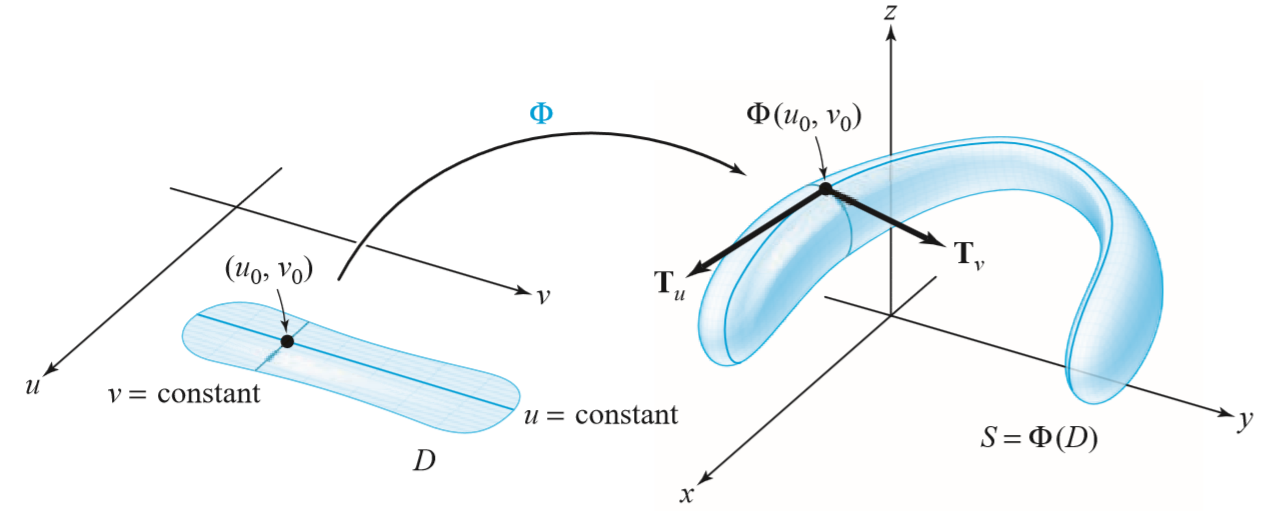
\includegraphics[width = 0.7\linewidth]{imagenes/phi.jpg}
\end{figure}

Al igual que pasaba con la parametrización de curvas, en superficies existe una orientación exterior e interior. Si $(\textbf{T}_{\textbf{u}_\textbf{0}} \times \textbf{T}_{\textbf{v}_\textbf{0}})/\Vert \textbf{T}_{\textbf{u}_\textbf{0}} \times \textbf{T}_{\textbf{v}_\textbf{0}} \Vert =  n(\phi(u_0,v_0))$ donde $n()$ es la normal de la parametrización, entonces decimos que la parametrización preserva la orientación, mientras que si  $(\textbf{T}_{\textbf{u}_\textbf{0}} \times \textbf{T}_{\textbf{v}_\textbf{0}})/\Vert \textbf{T}_{\textbf{u}_\textbf{0}} \times \textbf{T}_{\textbf{v}_\textbf{0}}\Vert =  -n(\phi(u_0,v_0))$ entonces la parametrización invierte la orientación.

Por tanto, $\textbf{T}_\textbf{u}$ y $\textbf{T}_\textbf{v}$ forman el plano tangente a $S$ en $(u_0, v_0)$. Si $\textbf{T}_\textbf{u} \times \textbf{T}_\textbf{v} = 0$ entonces la superficie no es diferenciable en ese punto. Otra propiedad interesante de estos vectores es que si tomamos un vector $\textbf{p}$ y hallamos el producto mixto con $\textbf{T}_\textbf{u}$ y $\textbf{T}_\textbf{v}$, es decir, $\textbf{p}\cdot(\textbf{T}_\textbf{u}\times \textbf{T}_\textbf{v}) = \text{det}(\textbf{p}, \textbf{T}_\textbf{u}, \textbf{T}_\textbf{v})$ éste nos indica el volumen del paralelepípedo formado por estos tres vectores. Por otra parte, $\Vert \textbf{T}_\textbf{u}\times \textbf{T}_\textbf{v}\Vert$ indica el área que forman los vectores. Esto va a ser importante para el resto de integrales.


Teniendo en cuenta que $\Vert \textbf{T}_\textbf{u}\times \textbf{T}_\textbf{v}\Vert$ representa el área que forman $\textbf{T}_\textbf{u}$ y $\textbf{T}_\textbf{v}$, entonces, si tomamos porciones diferenciales $\d{u}$ y $\d{v}$, la integral de esas porciones se corresponderá con el área de la superficie. Así:
\[ A(S) = \int_D \Vert \textbf{T}_\textbf{u}\times \textbf{T}_\textbf{v} \Vert \d{u}\d{v}\]

Una superficie $z = f(x,y)$ puede modelarse como $(u,v,f(u,v))$, de modo que $\Vert \textbf{T}_\textbf{u}\times \textbf{T}_\textbf{v}\Vert = \sqrt{\left(\frac{\partial f}{\partial x}\right)^2 + \left(\frac{\partial f}{\partial y}\right)^2 + 1 }$.

Asimismo, podemos aplicar un valor a cada punto de la superficie $S$ con una función $f(x,y,z)$ y hallar la integral de $f$ sobre $S$. El valor de esta integral es:
\[\int_S f(x,y,z) dS = \int_D f(\Phi(u,v)) \Vert \textbf{T}_\textbf{u}\times \textbf{T}_\textbf{v} \Vert \d{u}\d{v} \]

Si por ejemplo $S$ puede representarse como una gráfica $z = g(x,y) = \Phi(x,y)$ entonces la integral de $f$ sobre $S$ sería:
\[\int_D f(x,y,g(x,y)) \Vert \textbf{T}_\textbf{x}\times \textbf{T}_\textbf{y} \Vert \d{x}\d{y} = \int_Df(x,y,g(x,y)) \sqrt{\left(\frac{\partial g}{\partial x}\right)^2 + \left(\frac{\partial g}{\partial y}\right)^2 + 1 } \d{x}\d{y}\]

Si en lugar de una función escalar tenemos un campo vectorial, también podríamos calcular la integral de superficie de F sobre $S$ o, mejor dicho, sobre la parametrización de la superficie $\Phi$. La intuición de esta integral es indicar la cantidad de ``campo'' que está atravesando la superficie. Por ejemplo, podemos imaginar el campo $F(x,y,z) = (x,y,0)$ que sería paralelo al plano $P \equiv z = 0$. Si tuviéramos una superficie en ese plano, la integral de superficie sería 0, porque ninguna ``flecha'' del campo vectorial atravesaría la superficie. La integral de superficie es máxima cuando las ``flechas'' del campo vectorial son perpendiculares a la superficie en todo momento.

Es importante considerar que las ``flechas'' tienen sentido, es decir, que se pueden anular entre sí. Si imaginamos el campo $F = (x,y,z)$ y la esfera unitaria, la integral total es 0, porque las flechas de octantes opuestos se anulan.

Así, el integral de superficie sobre un campo se define por:
\[\int_D \textbf{F} \cdot (\textbf{T}_\textbf{u}\times \textbf{T}_\textbf{v}) \d{u}\d{v}  \]

Al igual que pasaba con las integrales de línea, las integrales de campo son iguales independientemente de la parametrización de $S$. Es decir, si existen dos parametrizaciones de $S$, $\Phi_1$ y $\Phi_2$, entonces se cumple que 
\[\int_{\Phi_1} \textbf{F}\cdot \d{S} = \pm \int_{\phi_2} \textbf{F}\cdot \d{S}  \]
El signo más o menos dependerá de si las parametrizaciones tienen el mismo estado de inversión de la superficie, o si tienen diferentes estados.

Como último punto, cabe mencionar que 
\[\int_D \textbf{F}\cdot(\textbf{T}_\textbf{u}\times \textbf{T}_\textbf{v}) \d{u}\d{v} = \int_D \textbf{F}\cdot\frac{(\textbf{T}_\textbf{u}\times \textbf{T}_\textbf{v})}{\Vert \textbf{T}_\textbf{u}\times \textbf{T}_\textbf{v}\Vert} \Vert \textbf{T}_\textbf{u}\times \textbf{T}_\textbf{v}\Vert \d{u}\d{v} = \int_D(\textbf{F}\cdot \textbf{n})\Vert \textbf{T}_\textbf{u}\times \textbf{T}_\textbf{v}\Vert\d{u}\d{v} = \int_S (\textbf{F}\cdot \textbf{n}) \d{S}\]

Si se sabe de antemano $\textbf{n}$ y la integral de superficie, esta relación puede ahorrarnos tiempo de cálculo.
\end{document}